\documentclass[12pt]{article}

\usepackage[utf8x]{inputenc}%
\usepackage[romanian]{babel}%
\usepackage{multirow}%
\usepackage{color}%
\usepackage{algorithm}%
\usepackage{algorithmic}%
\usepackage{hyperref}%
\usepackage{natbib}%
\usepackage{amsmath}%
\usepackage{array}%
\usepackage{graphicx}%
%\usepackage{import}%
\usepackage{caption}%
\usepackage{subcaption}%
\usepackage{float}%
\usepackage[margin=1.2in]{geometry}%

\floatname{algorithm}{Algoritmul}

\renewcommand{\algorithmicforall}{\textbf{pentru toate}}
\renewcommand{\algorithmicdo}{\textbf{execută}}
\renewcommand{\algorithmicuntil}{\textbf{până când}}
\renewcommand{\algorithmicend}{\textbf{termină}}
\renewcommand{\algorithmicif}{\textbf{dacă}}
\renewcommand{\algorithmicelse}{\textbf{altfel}}
\renewcommand{\algorithmicfor}{\textbf{ciclu}}
\renewcommand{\algorithmicthen}{\textbf{atunci}}
\renewcommand{\algorithmicrepeat}{\textbf{repetă}}
\renewcommand{\algorithmicendfor}{\algorithmicend\ \algorithmicfor}

\renewcommand{\algorithmicrequire}{\textbf{Intrări:}}
\renewcommand{\algorithmicensure}{\textbf{Ieșire:}}


\title{Învățare Automată - Tema 1 \\ \textbf{Învățare prin recompensă:
    Cărămizi}}%
\author{Tudor Berariu \\ {\small Laboratorul AIMAS} \\ {\small
    Facultatea de Automatică și Calculatoare}}%

\newcommand{\piesa}[2]{
    \hline%
    \begin{minipage}[t]{0.25\linewidth}%
      \begin{center}%
        \vspace{4pt}%
        #1%
        \vspace{4pt}%
      \end{center}%
    \end{minipage}%
    &
    \begin{minipage}[t]{0.5\linewidth}%
      \begin{center}%
        \vspace{4pt}%
        \includegraphics{graphics/piesa#2.pdf}%
        \vspace{4pt}%
      \end{center}%
    \end{minipage}%
      \\
}

\newcommand{\piesas}[1]{%
  \begin{minipage}[t]{0.15\linewidth}%
    \begin{center}%
      \vspace{3pt}%
      \includegraphics{graphics/piesa#1.pdf}%
      \vspace{3pt}%
    \end{center}%
  \end{minipage}
  }

\definecolor{blue(pigment)}{rgb}{0.2, 0.2, 0.6}
\newcommand{\sarsa}{{\color{blue(pigment)} \textbf{SARSA}}}
\newcommand{\qlearn}{{\color{blue(pigment)} $Q$\textbf{-learning}}}

\definecolor{darkygray}{rgb}{0.21, 0.21, 0.21}
\newcommand{\caramizi}{{\color{darkygray} \textbf{Cărămizi}}}
\newcommand{\engl}{{\color{darkygray}engl. }}

\begin{document}
\maketitle%

\section{Pe scurt...}
\label{sec:short}

Se cere să se implementeze algoritmul \sarsa{} pentru învățarea unei
strategii de joc pentru o variantă a jocului Tetris. Se va testa
eficiența algoritmului pentru diferite niveluri de complexitate a
jocului.

\section{Motivația temei}
\label{sec:motivation}

Scopul acestei teme îl reprezintă familiarizarea cu un algoritm de
învățare prin recompensă, \sarsa{}, precum și implementarea
acestuia. Se urmărește înțelegerea diferențelor dintre acesta și
algoritmul \qlearn, precum și aplicarea \sarsa{} pe o problemă în
care numărul stărilor este foarte mare.

\section{Descrierea jocului}
\label{sec:intro}

Jocul \caramizi{} este o variantă a jocului Tetris concepută
pentru studenții cursului de Învățare Automată cu o listă de
modificări descrisă în cele ce urmează.

Se consideră o fântână reprezentată ca un spațiu de înălțime $H$ și
lățime $W$ și 7 tipuri de cărămizi, enumerate în
Tabela~\ref{table:bricks}.

\begin{table}[h!]
  \centering
  \begin{tabular}{| c | c |}
    \piesa{A}{1}
    \piesa{B}{2}
    \piesa{C}{3}
    \piesa{D}{4}
    \piesa{E}{5}
    \piesa{F}{6}
    \piesa{G}{7}
    \hline
  \end{tabular}
  \caption{Tipurile de cărămizi}
  \label{table:bricks}
\end{table}

\subsection{Obiectivul jucătorului}
\label{sec:players}

Jucătorul, denumit de aici înainte \textbf{Meșter}, este cel care
așează cărămizile primite în fântână. Scopul lui este să formeze linii
orizontale complete pentru a obține un punctaj cât mai mare.

Meșterul va așeza cărămizile primite în fântână unele peste altele. O
cărămidă va putea fi așezată doar deasupra celor fixate deja. Spre
deosebire de Tetris clasic, aici cărămida va fi întâi rotită și
așezată deasupra poziției dorite și abia apoi lăsată să cadă fără a
mai fi deplasată sau rotită până ajunge jos (vezi
Figura~\ref{fig:incorrect}).

\begin{figure}[h!]
        \centering
        \begin{subfigure}[t]{0.25\textwidth}
                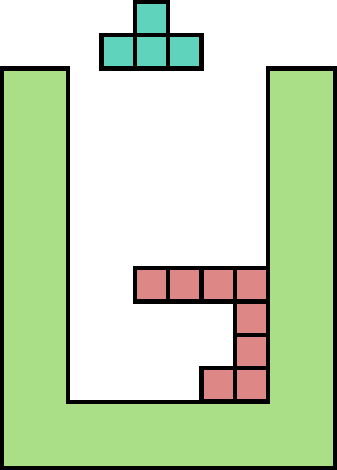
\includegraphics[width=\textwidth]{graphics/placenewA.pdf}
                \caption{Cărămida turcoaz trebuie așezată}
                \label{fig:incorrectA}
        \end{subfigure}%
        \qquad
        ~ %add desired spacing between images, e. g. ~, \quad, \qquad etc.
          %(or a blank line to force the subfigure onto a new line)
        \begin{subfigure}[t]{0.25\textwidth}
                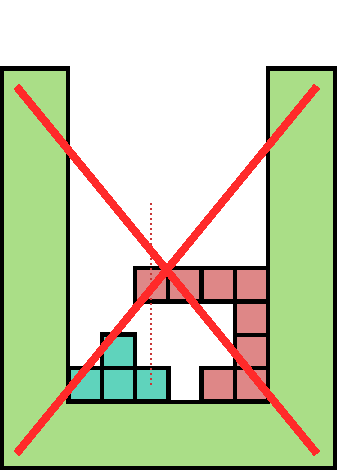
\includegraphics[width=\textwidth]{graphics/placenewB.pdf}
                \caption{Nu se poate așeza dacă deasupra ei nu este liber}
                \label{fig:incorrectB}
        \end{subfigure}%
        \caption{Exemplu de așezare incorectă a unei cărămizi}%
        \label{fig:incorrect}%
\end{figure}

Jocul se încheie atunci când au fost așezate \textbf{24} cărămizi sau
atunci când construcția depășește înălțimea $H$.

\subsection{Punctarea}
\label{sec:scoring}

Atunci când în urma așezării unei cărămizi se completează una sau mai
multe linii, acestea vor dispărea (\emph{magie!}) și Meșterul va
primi:
\begin{itemize}
\item 1 punct pentru o linie completată,
\item 3 puncte pentru 2 linii completate,
\item 9 puncte pentru 3 linii completate,
\item 27 puncte pentru 4 linii completate.
\end{itemize}
Liniile completate nu trebuie să fie consecutive (vezi exemplul din
Figura~\ref{fig:complete}).

\begin{figure}[h!]
  \centering
  \begin{subfigure}[t]{0.23\textwidth}
    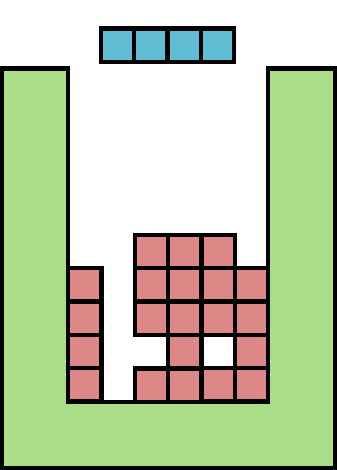
\includegraphics[width=\textwidth]{graphics/threelinesA.pdf}
    \caption{Cărămida turcoaz trebuie așezată}
    \label{fig:threelinesA}
  \end{subfigure}%
  ~ %add desired spacing between images, e. g. ~, \quad, \qquad etc.
  % (or a blank line to force the subfigure onto a new line)
  \begin{subfigure}[t]{0.23\textwidth}
    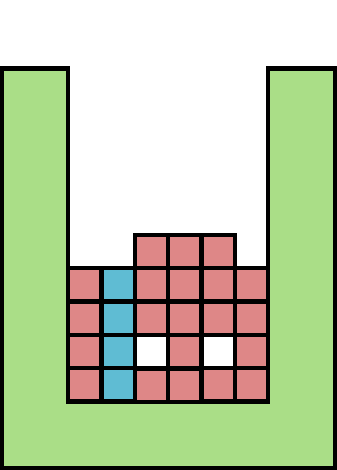
\includegraphics[width=\textwidth]{graphics/threelinesB.pdf}
    \caption{O posibilitate de a așeza cărămida}
    \label{fig:threelinesB}
  \end{subfigure}%
  ~ %add desired spacing between images, e. g. ~, \quad, \qquad etc.
  % (or a blank line to force the subfigure onto a new line)
  \begin{subfigure}[t]{0.23\textwidth}
    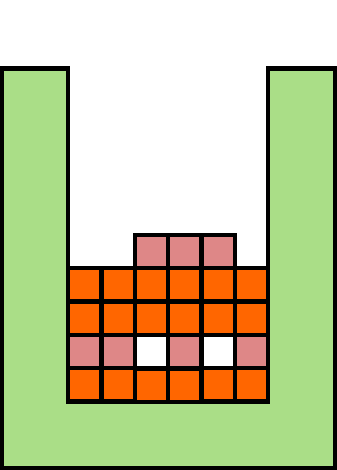
\includegraphics[width=\textwidth]{graphics/threelinesC.pdf}
    \caption{Cele trei linii aduc 9 puncte Meșterului}
    \label{fig:threelinesC}
  \end{subfigure}%
  ~ %add desired spacing between images, e. g. ~, \quad, \qquad etc.
  % (or a blank line to force the subfigure onto a new line)
  \begin{subfigure}[t]{0.23\textwidth}
    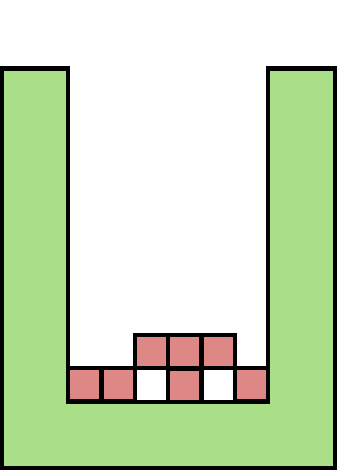
\includegraphics[width=\textwidth]{graphics/threelinesD.pdf}
    \caption{Fântâna după dispariția liniilor completate}
    \label{fig:threeLinesD}
  \end{subfigure}%
  \caption{Exemplu de completare a liniilor}%
  \label{fig:complete}%
\end{figure}

Dacă jocul se încheie prin depășirea înălțimii fântânii, atunci
Meșterului i se vor retrage 20 de puncte.

Toate regulile de punctare sunt trecute în Tabela~\ref{table:scoring}.

\begin{table}[h]
  \centering
  \begin{tabular}{| l | c | c |}
    \hline Eveniment & Puncte Meșter \\
    \hline 1 linie completată & 1  \\
    \hline 2 linii completate & 3  \\
    \hline 3 linii completate & 9  \\
    \hline 4 linii completate & 27 \\
    \hline Depășirea înălțimii fântânii & -20 \\
    \hline
  \end{tabular}
  \caption{Punctarea}
  \label{table:scoring}
\end{table}

\section{Algoritmul SARSA}
\label{sec:sarsa-alg}


Algoritmul \sarsa{} (State-Action-Reward-State-Action)
\citep{rummery1994line,singh1996reinforcement} este similar
algoritmului \qlearn{}.

\begin{algorithm}
  \caption{Algoritmul SARSA}
  \begin{algorithmic}[1]
    \FORALL{stările $s$} \FORALL{acțiunile $a \in A(s)$} \STATE Q(s,a)
    $\longleftarrow$ 0
    \ENDFOR
    \ENDFOR
    \FORALL{episoadele} \STATE $s \longleftarrow$ stare inițială
    \STATE $a \longleftarrow$ $\epsilon$-greedy$(Q,s)$ \REPEAT \STATE
    execută $a$ \STATE observă $s',r$ \STATE $a' \longleftarrow$
    $\epsilon$-greedy$(Q,s')$ \STATE $Q(s,a) \longleftarrow Q(s,a) +
    \alpha \Big( r + \gamma Q(s',a') - Q(s,a) \Big)$ \STATE $s
    \longleftarrow s'$ \STATE $a \longleftarrow a'$ \UNTIL{$s$ este
      stare finală}
    \ENDFOR
  \end{algorithmic}
  \label{algsarsa}
\end{algorithm}

Regula de actualizare a funcției $Q$ este diferită față de cea a
algoritmului \qlearn{} (vezi Formula~\ref{eq:sarsa}) prin faptul că
pentru estimarea \emph{recompenselor viitoare} nu se alege întotdeauna
valoarea maximă pentru $Q(s',*)$, ci se alege o acțiune $a'$ conform
politicii (care include și componenta de explorare) și se utilizează
valoarea $Q(s',a')$. Din puncte de vedere conceptual, această
diferență se traduce prin faptul că \sarsa{} este un algoritm
\emph{on-policy} spre deosebire de \qlearn{} care este un algoritm
\emph{off-policy}.

Formula de actualizare a funcției $Q$ în algoritmul \sarsa{}:
\begin{equation}
  \label{eq:sarsa}
  Q_{t+1}(s_{t},a_{t}) \longleftarrow Q_{t}(s_{t},a_{t}) +
  \alpha_t \Big(R(s_{t},a_{t}) +
  \gamma Q_{t}(s_{t+1},a_{t+1})-Q_{t}(s_{t},a_{t})\Big)
\end{equation}

În cazul unui proces de învățare continuu este de așteptat ca
algoritmii on-policy să se comporte mai bine decât algoritmii
off-policy întrucât politica învățată ține cont și de componenta de
explorare. Acest lucru este util mai ales atunci când mediul este unul
dinamic și nu se poate renunța la explorare.

Avantajul algoritmului \sarsa{} față de \qlearn{} este foarte bine
surprinsă în următorul paragraf din \citep{baird1999reinforcement}:
\emph{$[\ldots]$ perhaps it would be better to learn the policy that
  is optimal, given that you will explore $\epsilon$ of the time. It
  would be like a person who, when walking, always takes a random step
  every 100 paces or so. Such a person would avoid walking along the
  top of a cliff, even when that is the optimal policy for a person
  who doesn't explore randomly.}

Pseudocodul \sarsa{} este prezentat în
Algoritmul~\ref{algsarsa}. Pentru alegerea acțiunii dintr-o stare $s$
folosiți tehnica $\epsilon$-greedy, descrisă de
Algoritmul~\ref{alg:epsilongreedy}.

\begin{algorithm}
  \caption{Algoritmul $\epsilon$-greedy}
  \begin{algorithmic}[1]
    \REQUIRE $Q$, starea $s$,$\epsilon$, $A$ \ENSURE acțiunea $a$
    \STATE $A' \longleftarrow \lbrace a \in A \vert a \text{ acțiune
      validă în } s \rbrace$ \STATE $p \longleftarrow random(0,1)$
    \IF{$p < \epsilon$} \STATE $a \longleftarrow random(A')$ \ELSE
    \STATE $a \longleftarrow \underset{act \in
      A'}{\operatorname{argmax}}$ $Q(s,act)$
    \ENDIF
  \end{algorithmic}
  \label{alg:epsilongreedy}
\end{algorithm}

\section{Cerințe}
\label{sec:tasks}

\subsection*{[6 puncte] Implementarea algoritmului \sarsa{}}
\label{sec:sarsa}

Să se implementeze algoritmul \sarsa{} pentru a determina o politică
(o strategie de joc) cât mai bună pentru \textbf{Meșter} în jocul
\caramizi. Se impune o optimizare a reprezentării
stărilor. Implementarea se poate face de la zero sau se pot folosi ca
punct de plecare serverul de joc și scripturile din arhivă (vezi
Anexa~\ref{sec:code}).

Se vor acorda 4 puncte pentru implementarea corectă a algoritmului și
2 puncte pentru optimizarea reprezentării stărilor. Compararea mai
multor reprezentări și studierea implicației fiecăreia asupra
învățării (scor obținut în urma învățării și timp necesar pentru
învățare) pot aduce punctaj suplimentar.

\subsection*{[4 puncte] Evaluarea eficienței algoritmului}
\label{sec:evaluation}

Se va evalua metoda de învățare propusă prin observarea scorului
obținut de \textbf{Meșter} de-a lungul unui număr mare de jocuri
(\textbf{Meșterul} își păstrează utilitățile de la un joc la altul)
pentru patru niveluri de dificultate a jocului.

Se vor realiza două grafice: unul cu evoluția scorului obținut de
\textbf{Meșter}, eventual netezit, și unul pentru evoluția numărului
de stări explorate pe parcursul învățării.

Se va testa algoritmul pentru cele patru cazuri descrise în Tabela
~\ref{table:opponents} și pentru unul la alegere.

\begin{table}[!h]
\centering
  \begin{tabular}{| l || c | c || c | c | r |}
    \hline
    \multirow{3}{*}{Nr} &
    \multicolumn{2}{ c ||}{Fântâna} &
    \multicolumn{3}{ c |}{Cărămizile} \\
    \cline{2-6} &
    \multirow{2}{*}{$H$} & \multirow{2}{*}{$W$} &
    Distribuția &
    % \multirow{2}{*}{Distribuția fixă?} &
    \multicolumn{2}{ c |}{Distribuția de probabilitate} \\
    \cline{5-6} & & & fixă? & Cărămida & Probabilitatea de apariție \\
    \hline
    \hline
    1 & 4 & 4 & Da & \piesas{1} & 1 \\
    \hline
    \hline
    \multirow{2}{*}{2} & \multirow{2}{*}{8} &
    \multirow{2}{*}{5} & \multirow{2}{*}{Da} &
    \piesas{1} & 0.5 \\
    \cline{5-6} & & & & \piesas{7} & 0.5 \\
    \hline
    \hline
    \multirow{3}{*}{3} & \multirow{3}{*}{8} &
    \multirow{3}{*}{5} & \multirow{3}{*}{Da} &
    \piesas{1} & 0.2 \\
    \cline{5-6} & & & & \piesas{2} & 0.4 \\
    \cline{5-6} & & & & \piesas{3} & 0.4 \\
    \hline
    \hline
    \multirow{4}{*}{4} &
    \multirow{4}{*}{8} &
    \multirow{4}{*}{6} &
    \multirow{4}{*}{Da} &
    \piesas{1} & 0.16667 \\
    \cline{5-6} & & & & \piesas{4} & 0.66665 \\
    \cline{5-6} & & & & \piesas{5} & 0.08334 \\
    \cline{5-6} & & & & \piesas{6} & 0.08334 \\
    \hline
  \end{tabular}
  \caption{Scenariile de test}
  \label{table:opponents}
\end{table}

Trebuie căutate valori cât mai bune pentru rata de învățare
($\alpha$), factorul de atenuare ($\gamma$) și probabilitatea de
explorare ($\epsilon$).

\subsection*{[2 puncte] BONUS}
\label{sec:bonus}

Faceți o comparație între algoritmul \sarsa{} și algoritmul \qlearn{}
pentru scenariile date. Aduce \sarsa{} vreun avantaj față de \qlearn{}
pentru învățarea on-line? Interpretați și explicați rezultatele
obținute.

\section{Trimiterea temei}
\label{sec:homework}

În arhiva temei includeți:
\begin{itemize}
\item toate fișierele sursă (cu \texttt{Makefile} / script de
  compilare și rulare)
\item fișier \texttt{pdf} cu descrierea implementării și a
  rezultatelor obținute:
  \begin{itemize}
  \item reprezentarea stărilor (eventual comparație făcută între mai
    multe reprezentări încercate);
  \item grafice cu scorul obținut pe parcursul învățării și cu numărul
    de stări pentru scenariile propuse;
  \item comparația (eventual grafice suprapuse) între \qlearn{} și
    \sarsa{}
  \end{itemize}
\end{itemize}

\appendix
\section{Arhiva}
\label{sec:code}

În arhiva ce însoțește acest document se găsește implementarea unui
server de joc pentru \caramizi. Pentru a folosi acest server de
joc la testarea temei trebuie să comunicați prin pipe-uri cu nume
(\engl{} \emph{named pipes}) respectând protocolul descris în
Figura~\ref{fig:protocol} și \emph{narat} în
Secțiunea~\ref{sec:protocol-story}.

\section{Conținutul arhivei}
\label{sec:archive}

\begin{itemize}
\item \texttt{src/} - sursele serverului;
\item \texttt{Makefile} - rețetele pentru compilarea serverului;
\item \texttt{delete\_pipes.sh} și \texttt{create\_pipes.sh} -
  scripturi pentru crearea și ștergerea pipe-urilor cu nume (denumite
  \texttt{server\_to\_player} și \texttt{player\_to\_server});
\item \texttt{distributions/} - director cu fișierele cu distribuțiile
  de probabilități de apariție a cărămizilor;
\item \texttt{start\_server.sh} - script pentru lansarea serverului
  pentru scenariile propuse în cerințe.
\end{itemize}

\subsection{Protocolul de comunicație}
\label{sec:protocol-story}

Toate mesajele schimbate de cele două entități (serverul de joc și
meșterul) se încheie cu \verb|\n|.

Serverul va controla evoluția jocului și îi va cere Meșterului să
poziționeze fiecare cărămidă.

Întâi jucătorul trebuie să se conecteze la server (adică să deschidă
cele două pipe-uri cu nume) și să trimită un mesaj cu numele lui
(\verb|MESHTER\n|). Drept răspuns va primi numărul de jocuri și
dimensiunea fântânii (de exemplu un mesaj \verb|100000,10,6\n|).

\begin{figure}[h!]
  \centering
  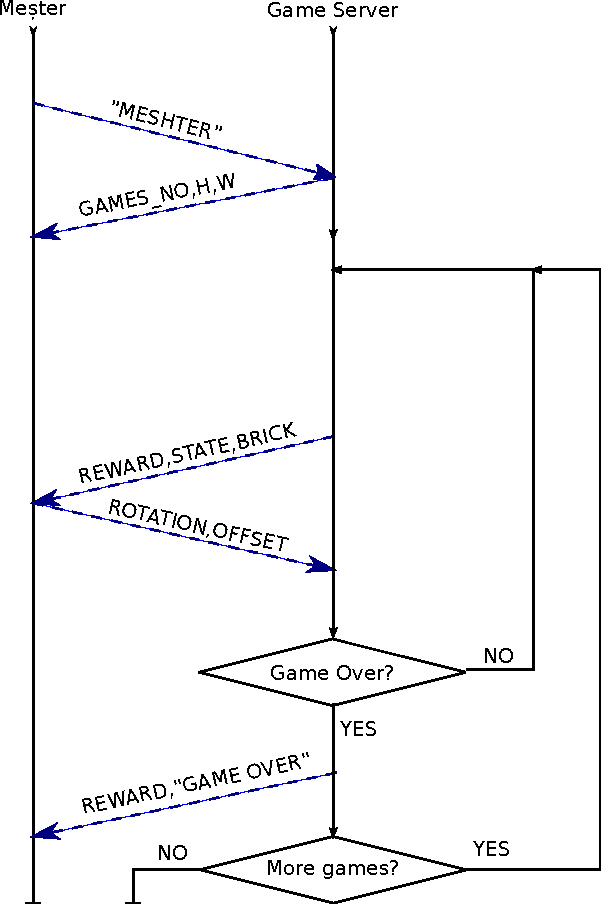
\includegraphics[width=0.4\textwidth]{graphics/protocol.pdf}
  \caption{Protocolul de comunicație}
\label{fig:protocol}
\end{figure}

Începând din acest moment, pentru fiecare joc:
\begin{enumerate}
\item serverul îi trimite Meșterului un mesaj ce conține numărul de
  puncte obținute pentru mutarea anterioară, starea jocului, dar și
  piesa ce trebuie poziționată. Un exemplu de mesaj este:
\begin{verbatim}
9,|    |    |   #|  ##|## #|,C\n
\end{verbatim}
\item Meșterul îi trimite serverului două numere: numărul de rotații
  în sensul acelor de ceasornic ce trebuie executate și numărul de
  celule distanță de la peretele din stânga. Un exemplu de mesaj este:
\begin{verbatim}
3,2\n
\end{verbatim}
  pentru o piesă rotită cu 270 de grade și care va fi plasată la
  distanță de 2 căsuțe de peretele din stânga (începând cu a treia
  coloană).
\item Dacă jocul s-a încheiat (s-au pus 24 piese sau s-a depășit
  înălțimea fântânii), serverul îi trimite Meșterului un mesaj cu
  ultimele puncte câștigate și textul \texttt{GAME OVER}. De exemplu:
\begin{verbatim}
27,GAME OVER\n
\end{verbatim}
\end{enumerate}

\subsection{Utilizarea fișierelor din arhivă}
\label{sec:scripts}

\begin{enumerate}
\item Se creează pipe-urile cu nume \texttt{server\_to\_player} și
  \texttt{player\_to\_server}:
\begin{verbatim}
$ ./delete_pipes
$ ./create_pipes
\end{verbatim}
\item Se lansează serverul de joc:
\begin{verbatim}
$ ./bricks-game-server --gamesNo 100 --height 8 --width 6 \
                       --bricks distributions/dist2 \
                       --verbose 1 --log STDOUT \
/
Starting server for 1 games on a 8x6 board.
Waiting for player...
\end{verbatim}
  \begin{itemize}
  \item Se pot configura:
    \begin{itemize}
    \item numărul de jocuri (\texttt{--gamesNo}), implicit 100000;
    \item dimensiunea fântânii (\texttt{--height} și
      \texttt{--width}), implicit $8\times 6$;
    \item fișierul ce conține distribuția folosită pentru generarea
      cărămizilor (\texttt{--bricks}), implicit
      \texttt{distributions/dist1};
    \item pipe-ul cu nume pentru comunicarea de la jucător către
      server (\texttt{--inFIFO}) implicit \texttt{player\_to\_server};
    \item pipe-ul cu nume pentru comunicarea de la server către
      jucător (\texttt{--outFIFO}) implicit
      \texttt{server\_to\_player};
    \item controlul afișării (\texttt{--verbose}), implicit 0 (fals);
    \item fișierul către care să se scrie evoluția jocului
      (\texttt{--log}), implicit \texttt{STDOUT}, adică afișare la
      ecran;
    \end{itemize}
  \end{itemize}
\item Se lansează jucătorul (într-un terminal separat):
\begin{verbatim}
$ ./bricks-game-player
\end{verbatim}
\end{enumerate}

Un Meșter care așează piesele aleator este implementat în
\texttt{bricks-game-player.cc}. Pentru rezolvarea temei se poate porni
de la codul din acest fișier.

Rulați \verb|./start_server <n>| pentru a rula scenariul cu numărul
\texttt{n}.

\bibliographystyle{alpha}%
\bibliography{tb_ml2015_t01.bib}%

\end{document}
